% Document type, global settings, and packages

\documentclass[12pt, openany]{report}   %12 point font for Times New Roman
\usepackage{graphicx}  %for images and plots
\usepackage[letterpaper, left=1in, right=1in, top=1in, bottom=1in]{geometry}
\usepackage{setspace}  %use this package to set linespacing as desired
\usepackage{times}  %set Times New Roman as the font
\usepackage[explicit]{titlesec}  %title control and formatting
\usepackage[titles]{tocloft}  %table of contents control and formatting
\usepackage[backend=bibtex, sorting=none, bibstyle=ieee]{biblatex}  %reference manager
\usepackage{appendix}  %for appendices
\usepackage{rotating}  %for rotated, landscape images
\usepackage[normalem]{ulem}  %for underlined section titles
\usepackage{textcomp} % for text symbols such as copyright etc. 
\usepackage{indentfirst} % To indent the first line of every paragraph
\usepackage{array,arydshln} %for better table formatting. 
\usepackage{amsmath} %for formula formatting
\usepackage[T1]{fontenc} % improved font encoding
\usepackage[utf8]{inputenc} % for better handling of non-ASCII characters
%\usepackage{newtxtext} % font choice
\usepackage{newtxmath} 
%\usepackage{lmodern} % font choice 
%\usepackage[bookmarks=true, hidelinks]{hyperref}
\usepackage[hidelinks]{hyperref}
\usepackage{datetime}
%\usepackage{lastpage}  % Add the lastpage package
\usepackage{refcount}
%\usepackage[acronym]{glossaries}
\usepackage[acronym,nomain,nonumberlist]{glossaries}
\usepackage{acronym}
\usepackage[font=bf]{caption}

\makeglossaries
% List acronyms you would like to have appear in the List of Abbreviations. 
% Each acronym is in the format \newacronym{tag}{acronym}{long}
% The "tag" field is used when defining the acronym in the main text. The "acronym" field  contains the abbreviated form, and the "log" field contains the unabbreviated definition.
% Note: in order for the acronym to appear in the List of Acronyms, it must be tagged in the main text.
% To tag the acronym in the main text, you can write something like:  \acrlong{dna} (abbreviated \acrshort{dna}) is the molecule that carries genetic information for the development and functioning of an organism.

\newacronym{dna}{DNA}{Deoxyribonucleic acid}

\newacronym{rna}{RNA}{Ribonucleic acid} %glossary terms, make glossary

% Bibliography
%Add your bibliography file here
\bibliography{references}

% prevent certain fields in references from printing in bibliography
\AtEveryBibitem{\clearfield{issn}}
\AtEveryBibitem{\clearlist{issn}}

\AtEveryBibitem{\clearfield{language}}
\AtEveryBibitem{\clearlist{language}}

\AtEveryBibitem{\clearfield{doi}}
\AtEveryBibitem{\clearlist{doi}}

\AtEveryBibitem{\clearfield{url}}
\AtEveryBibitem{\clearlist{url}}

\AtEveryBibitem{%
  \ifentrytype{online}
    {}
    {\clearfield{urlyear}\clearfield{urlmonth}\clearfield{urlday}}}


% Start of Dissertation Document

\begin{document}
\doublespacing  %set line spacing to double by default throughout the document. This can be overwritten when necessary

% Title Page (No page number)
\pagenumbering{gobble}
\newdateformat{monthyeardate}{%
\monthname[\THEMONTH] \THEYEAR}
  
\begin{titlepage}
\begin{center}

\begin{singlespacing}
\vspace*{2\baselineskip}

\includegraphics[width = 1.73 in]{figures/Rockefeller_Seal.jpg}\\
\vspace*{5\baselineskip}

TITLE OF THESIS\\ % Write your dissertation title in ALL CAPS. It should match the title given on the Abstract page.

\vspace{8\baselineskip}
A Thesis Presented to the Faculty of\\
The Rockefeller University\\
in Partial Fulfillment of the Requirements for\\
the degree of Doctor of Philosophy\\
\vspace{8\baselineskip}
by\\
Student Name\\ % Fill in your name here
Month and Year of Degree Conferral % Fill in the month and year of your degree conferral with no comma. For example: June 2024 
\vspace{3\baselineskip}
\vfill


\end{singlespacing}

\end{center}
\end{titlepage}




% Copyright  Page (No page number)
\pagenumbering{gobble}


%\begin{titlepage}
\begin{singlespacing}
\begin{center}

\vspace*{40\baselineskip}

\textcopyright \, by Student Name \the\year\\ % Fill in your name here.
\vspace{\baselineskip}	

\end{center}
\vfill

\end{singlespacing}
%\end{titlepage}


% Abstract (No page number)
\pagenumbering{gobble}
%Abstract Page
%\begin{titlepage}
\begin{center}
\thispagestyle{empty}

TITLE 

Student Name\\
The Rockefeller University \the\year
\end{center}
\begin{flushleft}
\hspace{10mm}
\textbf{(Insert abstract here, about 1.5 pages long)}

Lorem ipsum dolor sit amet, consectetur adipiscing elit. Sed consequat mollis urna id rhoncus. Fusce a faucibus nibh. Vivamus porta aliquet metus, efficitur posuere lectus dignissim at. Duis scelerisque sapien non volutpat pellentesque. Vivamus ullamcorper nec sapien et suscipit. Vestibulum tristique egestas lectus, id porta urna cursus in. Suspendisse ut ipsum libero. Proin quis blandit purus. Etiam blandit lacinia placerat.

Maecenas quis aliquet dui, eget cursus dui. Duis facilisis mauris eu urna iaculis finibus. Morbi ex tellus, vulputate sit amet lobortis fermentum, vulputate sit amet diam. Sed facilisis est id dictum volutpat. Pellentesque tempus lacus sit amet sem mattis molestie. Mauris id convallis mauris. Etiam ullamcorper finibus elit.

Donec lacinia pulvinar nibh et pretium. Suspendisse at rutrum quam. Phasellus blandit non eros non bibendum. Cras vitae gravida enim. Aenean nec est odio. Sed aliquet ante vitae nulla efficitur, ut hendrerit massa dictum. Sed vitae facilisis urna. Cras diam sem, pulvinar non ultrices at, molestie id nunc. Morbi rhoncus in leo quis eleifend. Donec eget est id quam aliquet imperdiet. Cras gravida nisi in nunc interdum, vitae hendrerit tortor ultricies. Morbi ut metus laoreet, consectetur risus a, finibus libero. Nunc iaculis urna metus, vel vehicula tellus consequat non. Donec at magna risus. Vivamus vitae interdum diam.

Nam et erat eros. Cras sed laoreet nulla. Curabitur malesuada metus non metus ultrices vehicula. Nullam sit amet urna neque. Cras consectetur libero libero, sit amet pulvinar risus commodo at. Phasellus vulputate vulputate ex, id condimentum est eleifend ac. Morbi convallis sed lacus non placerat. Nullam eros metus, tincidunt sit amet pellentesque eget, egestas eu dolor.

In vitae convallis tellus, vel cursus magna. Integer vulputate nulla eget lorem tempus gravida. Etiam finibus, orci ac lobortis laoreet, sem magna elementum dui, ut varius lacus massa ut libero. Nam pretium, nisl sit amet elementum semper, nisl arcu congue arcu, nec fermentum dolor neque sit amet nibh. Suspendisse vitae odio a metus tempus dapibus malesuada et lectus. Morbi massa augue, vulputate id purus eget, aliquam auctor ipsum. Aenean justo leo, suscipit posuere tincidunt in, ornare at urna. Donec tempus id sapien nec viverra.

Lorem ipsum dolor sit amet, consectetur adipiscing elit. Sed consequat mollis urna id rhoncus. Fusce a faucibus nibh. Vivamus porta aliquet metus, efficitur posuere lectus dignissim at. Duis scelerisque sapien non volutpat pellentesque. Vivamus ullamcorper nec sapien et suscipit. Vestibulum tristique egestas lectus, id porta urna cursus in. Suspendisse ut ipsum libero. Proin quis blandit purus. Etiam blandit lacinia placerat.

Maecenas quis aliquet dui, eget cursus dui. Duis facilisis mauris eu urna iaculis finibus. Morbi ex tellus, vulputate sit amet lobortis fermentum, vulputate sit amet diam. Sed facilisis est id dictum volutpat. Pellentesque tempus lacus sit amet sem mattis molestie. Mauris id convallis mauris. Etiam ullamcorper finibus elit.

Donec lacinia pulvinar nibh et pretium. Suspendisse at rutrum quam. Phasellus blandit non eros non bibendum. Cras vitae gravida enim. Aenean nec est odio. Sed aliquet ante vitae nulla efficitur, ut hendrerit massa dictum. Sed vitae facilisis urna. Cras diam sem, pulvinar non ultrices at, molestie id nunc. Morbi rhoncus in leo quis eleifend. Donec eget est id quam aliquet imperdiet. Cras gravida nisi in nunc interdum, vitae hendrerit tortor ultricies. Morbi ut metus laoreet, consectetur risus a, finibus libero. Nunc iaculis urna metus, vel vehicula tellus consequat non. Donec at magna risus. Vivamus vitae interdum diam.

\end{flushleft}
\vspace*{\fill}
\pagenumbering{gobble}
%\end{titlepage}


% Dedication
%\phantomsection
\clearpage
\pagenumbering{roman}
\setcounter{page}{3}
\addcontentsline{toc}{chapter}{Dedication}
%Dedication page. 
%This page is optional


\topskip0pt
\vspace*{\fill}
\begin{flushleft}
\textit{Type your dedication here. This page is optional.}
\end{flushleft}
\vspace*{\fill}
\clearpage
%\pagenumbering{gobble}  %remove page number on summary page




% Acknowledgments
\phantomsection
\addcontentsline{toc}{chapter}{Acknowledgments}
%ACKNOWLEDGEMENTS page. 
%This page is optional

%\clearpage
\begin{center}

%\vspace*{5\baselineskip}
\textbf{\large Acknowledgements}
\end{center}


\begin{flushleft}
\hspace{10mm} Write your acknowledgements here. The Acknowledgments may be written in the first person.
\end{flushleft}
%\clearpage

%\pagenumbering{gobble}  %remove page number on summary page





% Table of Contents
%\currentpdfbookmark{Table of Contents}{TOC}
% Format for Table of Contents
\renewcommand{\cftchapdotsep}{\cftdotsep}  %add dot separators
\renewcommand{\cftchapfont}{\normalfont}  %set title font weight that shows up on TOC
\renewcommand{\cftchappagefont}{}  %set page number font-weight
\renewcommand{\cftchappresnum}{Chapter }
\renewcommand{\cftchapaftersnum}{:}
\renewcommand{\cftchapnumwidth}{6em}
\renewcommand{\cftchapafterpnum}{\vskip\baselineskip} %set correct spacing for entries in single space environment
\renewcommand{\cftsecafterpnum}{\vskip\baselineskip}  %set correct spacing for entries in single space environment
\renewcommand{\cftsubsecafterpnum}{\vskip\baselineskip} %set correct spacing for entries in single space environment
\renewcommand{\cftsubsubsecafterpnum}{\vskip\baselineskip} %set correct spacing for entries in single space environment

%format title font size and position (this also applies to list of figures and list of tables)
\titleformat{\chapter}[display]
{\normalfont\bfseries\filcenter}{\chaptertitlename\ \thechapter}{0pt}{\large{#1}}

\renewcommand\contentsname{Table of Contents}
\begin{singlespace}
\tableofcontents
\setlength{\cftparskip}{\baselineskip}
\newpage
\phantomsection
\addcontentsline{toc}{chapter}{List of Figures}
\listoffigures
\newpage
\phantomsection
\addcontentsline{toc}{chapter}{List of Tables}
\listoftables
\newpage
\phantomsection
\addcontentsline{toc}{chapter}{List of Abbreviations}
%\printglossary[type=\acronymtype, title=List of Abbreviations, toctitle=List of Abbreviations]
\clearpage\begingroup\let\newpage\relax\printglossary[title=List of Abbreviations]\endgroup
\end{singlespace}
%%%%%%%
%	            %
% Chapters   %
%                   %
%%%%%%%

% General formatting for chapters, appendix, etc. 


% reset page numbering for rest of document 
\newpage
%\setcounter{page}{1} 


% Adjust chapter title formatting
\titleformat{\chapter}[display]
{\normalfont\bfseries\filcenter}{}{0pt}{\large\chaptertitlename\ \large\thechapter : \large\bfseries\filcenter{#1}}  
\titlespacing*{\chapter}
  {0pt}{0pt}{30pt}	%controls vertical margins on title
  
% Adjust section title formatting
\titleformat{\section}{\normalfont\bfseries}{\thesection}{1em}{#1}

% Adjust subsection title formatting
\titleformat{\subsection}{\normalfont}{\thesubsection}{0em}{\hspace{1em}#1}

% Below is a subsubsection, uncomment it if you need to use it
%\titleformat{\subsubsection}{\normalfont\itshape}{\thesubsection}{1em}{#1}

%%%%%%%%%%%%%%%%
% LaTeX tutorial chapter.
%%%%%%%%%%%%%%%%
\pagenumbering{arabic}
\chapter*{\LaTeX Tutorial}

The following is an introduction to some of the basic utilities of \LaTeX. While this tutorial may not answer all of your questions, the good news is that \LaTeX is widely used enough that the answer is probably out there somewhere! If you need additional help, you can consult:

\begin{itemize}
    \item Claire Warner (\url{cwarner@roclefeller.edu}) at the Rita \& Frits Markus Library
    \item Google! The internet is your friend, and it's almost guaranteed that someone has already asked your question before (and someone else has provided a solution). 
\end{itemize}

\section{Sections, Subsections, and Sub-Subsections} \label{sections}

You may want to organize your dissertation text by using a section hierarchy within your chapters. Sections, subsections, and sub-subsections will be automatically translated into the Table of Contents. Note that I have created a label for this section using the text. This means that if I want to reference Section \ref{sections} in other parts of the text, I can do so easily. This can also be done for subsections. If you swap the order of the sections in your text, all of the references will automatically have their numbers corrected.

\subsection{Subsection}

This is a subsection.

\subsubsection{Sub-Subsection}

This is a sub-subsection.

\section{Citing References}

You can cite references throughout your thesis. \LaTeX makes this easy through the use of a .bib file. The file called \url{references.bib} is where you will put all of the citations that you would like to reference in the main text of your dissertation. The references are in BibTeX format within the .bib file. There are several ways to automatically format references in this style:

\begin{enumerate}
    \item Use the Google Scholar Chrome extension. You can search for the desired article, click on ``Cite'' and select the BibTeX option. This will open a tab of plain text that can be copied and pasted into the .bib file.
    \item Use citation management software and export the desired citation(s) in BibTeX format. Note that while Zotero and Mendeley will do this easily, EndNote can cause more problems and will not automatically generate convenient citation keys. Once you have exported the citations, copy the text into the .bib file or upload the new file (if you do this, be sure to change the .bib file referenced in the main \url{thesis.tex} file).
    \item Link your citation manager directly to Overleaf. You can use this feature with either Mendeley or Zotero.
\end{enumerate}

Note that the references can be put into the .bib file in any order - they will automatically be formatted in the correct order when the References section is generated. To cite a reference in the text, simply type \url{\cite{key}}. Here, \url{key} is the citation key defined in the .bib entry for that citation. To cite multiple references at once, type \url{\cite{key1, key2}}. For example, \cite{anderson1995observation, schill2019water} and \cite{watson1953molecular} are the references used in this tutorial.

References will be enumerated in order of the first time they are cited. Citing them later in the text will maintain this numbering scheme and show the original citation number, like so: \cite{anderson1995observation}.

\section{Acronyms and Abbreviations}

You can add acronyms to the main text by writing something like the following: \acrlong{dna} (abbreviated \acrshort{dna}) is the molecule that carries genetic information for the development and functioning of an organism. This will populate the referenced acronym into the List of Acronyms in the front matter of your dissertation. Note that you must add the acronym to the \url{Abbreviations.tex} file \textbf{and} refer to it in the main text by its defined tag for it to appear in the List of Acronyms. The acronyms/abbreviations will appear listed in alphabetical order. Note that the List of Acronyms is an optional component of your dissertation. If you do not include it, be sure to define any acronyms or abbreviations where necessary in the text for clarity.

\section{Footnotes}

Here is an example of how to use footnotes. It is possible to write footnotes directly in the text itself \footnote{And type your footnote here.}. Or, mark the location of a footnote with footnote mark command\footnotemark \, and write the footnote on its own line. 

\footnotetext{Use the footnotetext command and write your footnote as previously.}

\section{Figures and Tables}

Figures and tables are important ways of visualizing data and conveying information. As always, be sure to cite figures and tables if they are not your own work, or if they have been featured in previous publications. \LaTeX provides environments for both figures and tables. Within each environment, you can specify the image file (or table contents and layout) as well as the title and caption. 

\subsection{Figures}

% This is a figure. Copy and paste this block of code for each figure. Change the width, image file path, title, and caption as needed. 
\begin{figure}
\begin{center}
	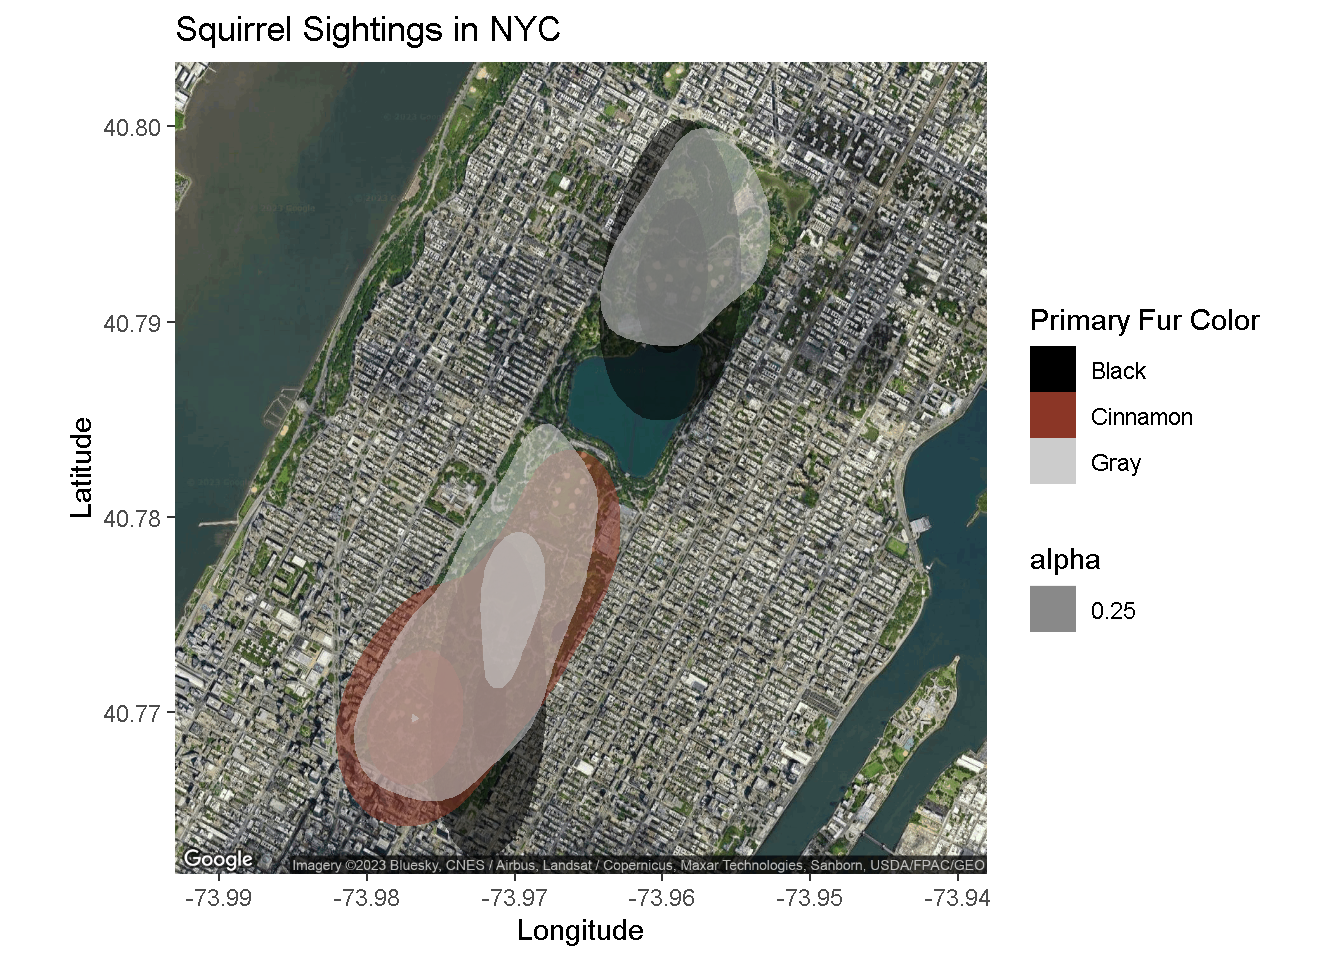
\includegraphics[width=0.8\textwidth]{figures/SquirrelData.png} % Adjust width and file path as needed.
	\caption[Figure title for the List of Figures]{ 
    Figure title for the main text. % By default, this should be identical to the figure title used in the List of Figures.
    \textmd{Type a longer subtitle or caption here, optionally, which will appear unbolded in the main text. This figure, sourced from \cite{squirreldata}, shows the geographical distribution of squirrels by fur color from the 2018 Central Park squirrel census.}
    }
    \label{fig:figurelabel} % Refer to this figure in the main text by typing \ref{figurelabel}. Be sure to give each figure a unique and sensible label.
    \end{center}
\end{figure}

You should try to include figures close to where they are discussed in the text. You can refer to any figure, such as Figure \ref{fig:figurelabel}, in the text. Note that if you switch the order in which figures are included in your \LaTeX code, the references in the text will automatically have their numbers updated. You may wish to organize your image files in sub-folders. To do this, you can create sub-folders (for example, by chapter) within the ``figures'' folder and adjust the file path accordingly when using the \url{\includegraphics} command.

Any figures you define will automatically be added to the List of Figures, and if their numbers or page locations change, this will be automatically updated when the file is compiled.



\subsection{Tables}

% This is a table
% Adapt the number of figures and columns as needed.
\begin{table}
\caption[Table title for the List of Tables]{ 
    Table title for the main text. % By default, this should be identical to the table title used in the List of Tables.
    \textmd{Type a longer subtitle or caption here, optionally, which appears unbolded in the main text. This table shows some common single-variable functions and their derivatives.}
    }\begin{center}
\begin{tabular}{ccc}
Function & Form & $x$-derivative \\
\hline
Constant & $a$ & 0 \\
Linear & $ax + b$ & $a$  \\
Quadratic & $ax^2 + bx + c$ & $2ax + b$  \\
\label{tab:tablelabel}
\end{tabular}
\end{center}
\end{table}

Tables are another important format for conveying both quantitative and qualitative information. First, begin the table environment using \url{\ begin{table} ... \ end{table}}. You can then define the titles for the List of Tables and the main text in the same way as was done for figures. To begin to input the table, you must create a second environment called \url{tabular}. Immediately after the \url{\ begin{tabular}} command, you will define the shape of the table and the text alignment within the cells. In the example table shown, \url{ {ccc} } specifies three columns with centered text and no vertical lines dividing them. To align the text left or right in a given column, simply type \url{l} or \url{r} instead of \url{c}. To place a vertical line between two columns, or on the edge of a column, use the ``|'' character in the appropriate location. For example, a table with a left- and a right-aligned column with borders and dividing lines would be defined by \url{ {|l|r|} }. 

You can then start filling in the contents of your table. The \url{&} character separates columns, and a double backslash indicates moving on to the line below. Typing \url{\ hline} will generate a horizontal line in your table. You can include equations or math characters in tables using \url{$ ... $}. You can further customize tables by merging columns or cells arbitrarily using the \url{\ multicolumn} command. If you are designing a complicated table, there are also many online tools that allow you to sketch out a table and generate the corresponding \LaTeX code! As discussed in the following section, you can refer to tables, such as Table \ref{tab:tablelabel}, in the main text using the \url{\ ref{}} command.

\section{Labels}

Labels are an extremely useful feature of \LaTeX. They can be added to figures, tables, equations, or sections so that the labeled item can be referenced later in the text. To label an item, simply type \url{\ label{yourlabelhere}}. For large documents such as a dissertation, it can be helpful to develop a sensible naming scheme and to categorize your labels by type. For example, label your figures \url{\ label{fig:yourfiglabelhere}} and tables \url{\ label{tab:yourtablabelhere}}. This will help ensure you choose the right label when referencing items. To reference the figure number defined previously, simply type \url{\ ref{fig:yourfiglabelhere}}. As discussed in the next section, the method for referencing equations is slightly different and uses the \url{\ eqref{}} command. If you later decide to swap the order of two figures, \LaTeX will automatically update the numbers referenced throughout the text.

\section{Math and Equations}

One of the very best things about the \LaTeX language is its ability to format mathematical equations just the way you like them, with extensive options for mathematical symbols, Greek letters, super- and subscripts, and other special characters or mathematical operators. It also uses the same reference system as figures and tables, so that equations can be numbered and given a label that can be referenced throughout the text. Let's take a look at the Schrodinger Equation.

\begin{equation}
    i \hbar \frac{\partial \Psi }{\partial t} = \hat{H} \Psi
    \label{eq:schrodinger}
\end{equation}

From this one example, you can see a hint of the power provided by \LaTeX for equation editing. For more information on how to format equations, see this \href{https://en.wikibooks.org/wiki/LaTeX/Mathematics}{link}. You can reference equations like Equation \eqref{eq:schrodinger} like so. 

You may also like to use mathematical symbols in line with the main text. To do this, simply use the dollar sign to create a mini-math environment. Then you can easily discuss $\alpha$ cells, $\beta$-keratins, or $\gamma$-rays without skipping a beat.

\section{\LaTeX Quirks}

\subsection{Quotation Marks}

Since \LaTeX is a compiled typesetting language, it doesn't do some things that other software, such as Microsoft Word, might do automatically. One subtle but important example of this is quotation marks. While Microsoft Word will automatically format left- and right-facing quotation marks as needed, in \LaTeX you will need to distinguish between them with separate characters, as shown here for ``double quotes'' and `single quotes'. Note that the right-side double quote is created using two apostrophes ('') rather than the double quote character ("). 

\subsection{Special Characters}

You may quickly find that in writing your dissertation, you would like to use a character that is also used in the \LaTeX coding language. For example, the percent sign % will begin a comment
and the ampersand symbol lets you align text in equations. If you would like to use these, or other, special characters in your text, simply use a backslash, like so: \% \&. 

\section{Useful Resources}

\begin{itemize}
    \item \href{https://www.overleaf.com/learn}{Overleaf Documentation}
    \begin{itemize}
        \item \href{https://www.overleaf.com/learn/how-to}{How-To Guides}
        \item \href{https://www.overleaf.com/learn/latex/Bibliography_management_with_bibtex}{BibTeX}
    \end{itemize}
    \item \href{https://tex.stackexchange.com/}{\LaTeX Stack Exchange}
    \item \href{https://en.wikibooks.org/wiki/LaTeX}{\LaTeX Wiki}
    \begin{itemize}
        \item \href{https://en.wikibooks.org/wiki/LaTeX/Chemical_Graphics}{Chemical Diagrams}
        \item \href{https://en.wikibooks.org/wiki/LaTeX/Special_Characters}{Special Characters}
        \item \href{https://en.wikibooks.org/wiki/LaTeX/Mathematics}{Math and Equation Notation}
    \end{itemize}
\end{itemize}

As always, you can contact Claire Warner (me!) in the Rockefeller University's Markus Library at \url{cwarner@rockefeller.edu} if you are having any trouble with this template! % Comment out this line to hide the tutorial

%%%%%%%%%%%%%%%%
% Chapter 1
%%%%%%%%%%%%%%%%

\chapter{Introduction and Background}

Given a set of numbers, there are elementary methods to compute 
its \acrlong{gcd}, which is abbreviated \acrshort{gcd}. This process 
is similar to that used for the \acrfull{lcm}

Lorem ipsum dolor sit amet, consectetur adipiscing elit, sed do eiusmod tempor incididunt ut labore et dolore magna aliqua. Ut enim ad minim veniam, quis nostrud exercitation ullamco laboris nisi ut aliquip ex ea commodo consequat \cite{ref1}. Duis aute irure dolor in reprehenderit in voluptate velit esse cillum dolore eu fugiat nulla pariatur \cite{ref2}. Excepteur sint occaecat cupidatat non proident, sunt in culpa qui officia deserunt mollit anim id est laborum.Lorem ipsum dolor sit amet, consectetur adipiscing elit, sed do eiusmod tempor incididunt ut labore et dolore magna aliqua. Ut enim ad minim veniam, quis nostrud exercitation ullamco laboris nisi ut aliquip ex ea commodo consequat \cite{ref1}. Duis aute irure dolor in reprehenderit in voluptate velit esse cillum dolore eu fugiat nulla pariatur

\section{Footnotes: Two ways of adding to your text}

Here is an example of how to use footnotes. It is possible to write footnotes directly in the text itself \footnote{By using footnote command and writing your note in the curly brackets}. Or it is possible to mark the location of a foot note with footnote mark command\footnotemark \, then you can write the footnote in its own line for ease of reading. 

\footnotetext{You then use footnotetext command and then write you note in as if you are using regular footnote command as we did previously.}

\section{Other section of first chapter}

Lorem ipsum dolor sit amet, consectetur adipiscing elit, sed do eiusmod tempor incididunt ut labore et dolore magna aliqua. Ut enim ad minim veniam, quis nostrud exercitation ullamco laboris nisi ut aliquip ex ea commodo consequat \cite{ref1}. Duis aute irure dolor in reprehenderit in voluptate velit esse cillum dolore eu fugiat nulla pariaturLorem ipsum dolor sit amet, consectetur adipiscing elit, sed do eiusmod tempor incididunt ut labore et dolore magna aliqua. Ut enim ad minim veniam, quis nostrud exercitation ullamco laboris nisi ut aliquip ex ea commodo consequat \cite{ref1}. Duis aute irure dolor in reprehenderit in voluptate velit esse cillum dolore eu fugiat nulla pariaturLorem ipsum dolor sit amet, consectetur adipiscing elit, sed do eiusmod tempor incididunt ut labore et dolore magna aliqua. Ut enim ad minim veniam, quis nostrud exercitation ullamco laboris nisi ut aliquip ex ea commodo consequat \cite{ref1}. Duis aute irure dolor in reprehenderit in voluptate velit esse cillum dolore eu fugiat nulla pariatur

Lorem ipsum dolor sit amet, consectetur adipiscing elit, sed do eiusmod tempor incididunt ut labore et dolore magna aliqua. Ut enim ad minim veniam, quis nostrud exercitation ullamco laboris nisi ut aliquip ex ea commodo consequat \cite{ref1}. Duis aute irure dolor in reprehenderit in voluptate velit esse cillum dolore eu fugiat nulla pariaturLorem ipsum dolor sit amet, consectetur adipiscing elit, sed do eiusmod tempor incididunt ut labore et dolore magna aliqua. Ut enim ad minim veniam, quis nostrud exercitation ullamco laboris nisi ut aliquip ex ea commodo consequat \cite{ref1}. Duis aute irure dolor in reprehenderit in voluptate velit esse cillum dolore eu fugiat nulla pariatur

Lorem ipsum dolor sit amet, consectetur adipiscing elit, sed do eiusmod tempor incididunt ut labore et dolore magna aliqua. Ut enim ad minim veniam, quis nostrud exercitation ullamco laboris nisi ut aliquip ex ea commodo consequat \cite{ref1}. Duis aute irure dolor in reprehenderit in voluptate velit esse cillum dolore eu fugiat nulla pariaturLorem ipsum dolor sit amet, consectetur adipiscing elit, sed do eiusmod tempor incididunt ut labore et dolore magna aliqua. Ut enim ad minim veniam, quis nostrud exercitation ullamco laboris nisi ut aliquip ex ea commodo consequat \cite{ref1}. Duis aute irure dolor in reprehenderit in voluptate velit esse cillum dolore eu fugiat nulla pariatur

Lorem ipsum dolor sit amet, consectetur adipiscing elit, sed do eiusmod tempor incididunt ut labore et dolore magna aliqua. Ut enim ad minim veniam, quis nostrud exercitation ullamco laboris nisi ut aliquip ex ea commodo consequat \cite{ref1}. Duis aute irure dolor in reprehenderit in voluptate velit esse cillum dolore eu fugiat nulla pariatur


% This is a figure. Copy and paste this block of code for each figure. Change the width, image file path, title, and caption as needed. 
\begin{figure}
	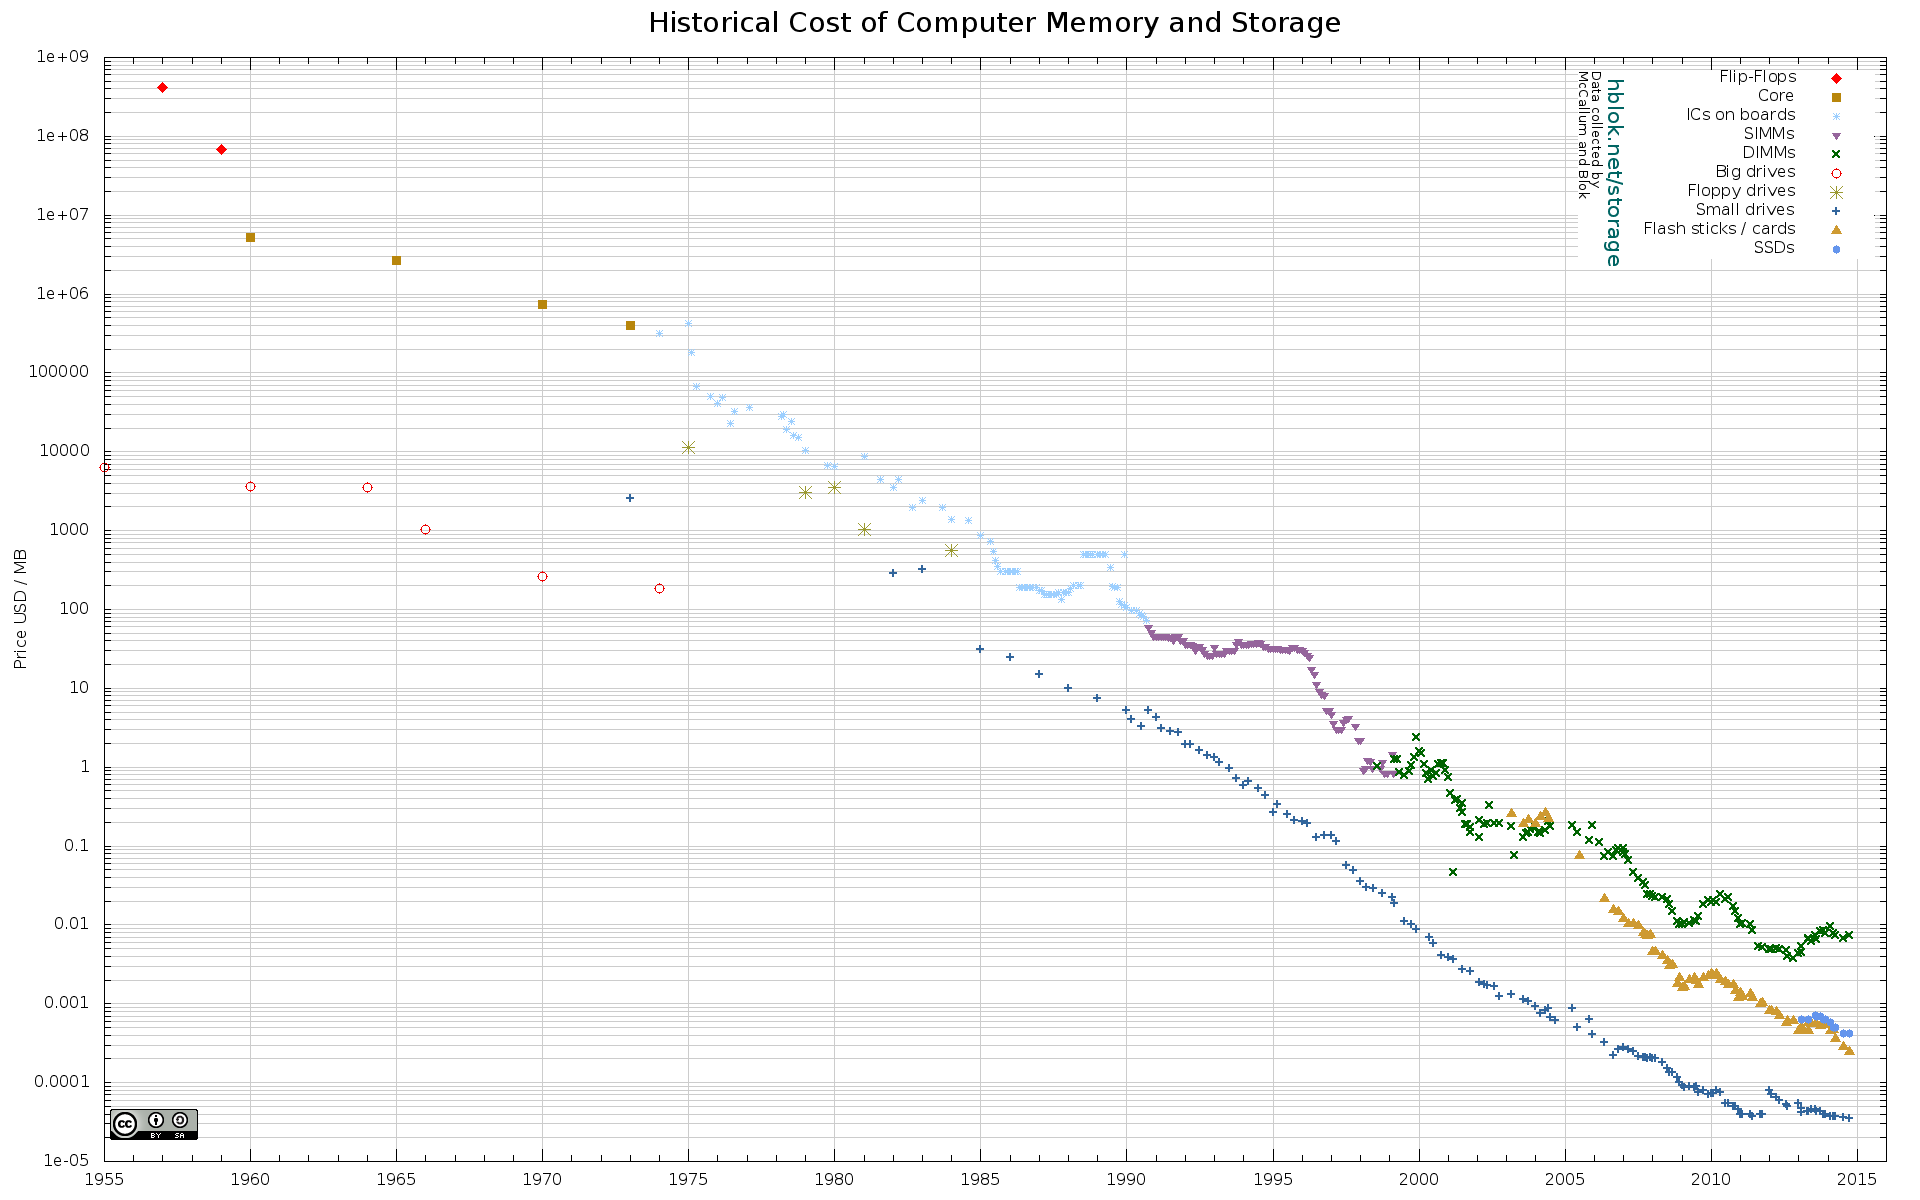
\includegraphics[width=\textwidth]{figures/exampleFigure.png} % Adjust width and file path as needed.
	\caption[Figure title for the Table of Contents]{ 
    Figure title for the main text. % By default, this should be identical to the figure title used in the Table of Contents.
    \textmd{Type a longer subtitle or caption here, optionally, which appears unbolded in the main text.}
    }
	\label{figurelabel} % Refer to this figure in the main text by typing \ref{figurelabel}. Be sure to give each figure a unique and sensible label.
\end{figure}



Lorem ipsum dolor sit amet, consectetur adipiscing elit, sed do eiusmod tempor incididunt ut labore et dolore magna aliqua. Ut enim ad minim veniam, quis nostrud exercitation ullamco laboris nisi ut aliquip ex ea commodo consequat \cite{ref1}. Duis aute irure dolor in reprehenderit in voluptate velit esse cillum dolore eu fugiat nulla pariatur \cite{ref2}. Excepteur sint occaecat cupidatat non proident, sunt in culpa qui officia deserunt mollit anim id est laborum \cite{ref3}.

Lorem ipsum dolor sit amet, consectetur adipiscing elit, sed do eiusmod tempor incididunt ut labore et dolore magna aliqua. Ut enim ad minim veniam, quis nostrud exercitation ullamco laboris nisi ut aliquip ex ea commodo consequat \cite{ref1}. Duis aute irure dolor in reprehenderit in voluptate velit esse cillum dolore eu fugiat nulla pariatur \cite{ref2}. Excepteur sint occaecat cupidatat non proident, sunt in culpa qui officia deserunt mollit anim id est laborum.

Lorem ipsum dolor sit amet, consectetur adipiscing elit, sed do eiusmod tempor incididunt ut labore et dolore magna aliqua. Ut enim ad minim veniam, quis nostrud exercitation ullamco laboris nisi ut aliquip ex ea commodo consequat \cite{ref1}. Duis aute irure dolor in reprehenderit in voluptate velit esse cillum dolore eu fugiat nulla pariatur \cite{ref2}. Excepteur sint occaecat cupidatat non proident, sunt in culpa qui officia deserunt mollit anim id est laborum.

Lorem ipsum dolor sit amet, consectetur adipiscing elit, sed do eiusmod tempor incididunt ut labore et dolore magna aliqua. Ut enim ad minim veniam, quis nostrud exercitation ullamco laboris nisi ut aliquip ex ea commodo consequat \cite{ref1}. Duis aute irure dolor in reprehenderit in voluptate velit esse cillum dolore eu fugiat nulla pariatur \cite{ref2}. Excepteur sint occaecat cupidatat non proident, sunt in culpa qui officia deserunt mollit anim id est laborum.

Lorem ipsum dolor sit amet, consectetur adipiscing elit, sed do eiusmod tempor incididunt ut labore et dolore magna aliqua. Ut enim ad minim veniam, quis nostrud exercitation ullamco laboris nisi ut aliquip ex ea commodo consequat \cite{ref1}. Duis aute irure dolor in reprehenderit in voluptate velit esse cillum dolore eu fugiat nulla pariatur \cite{ref2}. Excepteur sint occaecat cupidatat non proident, sunt in culpa qui officia deserunt mollit anim id est laborum.

Lorem ipsum dolor sit amet, consectetur adipiscing elit, sed do eiusmod tempor incididunt ut labore et dolore magna aliqua. Ut enim ad minim veniam, quis nostrud exercitation ullamco laboris nisi ut aliquip ex ea commodo consequat \cite{ref1}. Duis aute irure dolor in reprehenderit in voluptate velit esse cillum dolore eu fugiat nulla pariatur \cite{ref2}. Excepteur sint occaecat cupidatat non proident, sunt in culpa qui officia deserunt mollit anim id est laborum.

% This is a table
%If you are having issues with \midline use \hline insteadn and remove booktabs package from thesis.tex

\begin{table}
\caption{This is an example Table.}
\begin{center}
\begin{tabular}{ccc}
x & f(x) & g(x) \\
%\hline
\midrule
1 & 6 & 4  \\
2 & 6 & 3  \\
3 & 6 & 2  \\
4 & 6 & 2  \\
\label{Table in Chapter 1}
\end{tabular}
\end{center}
\end{table}



%%%%%%%%%%%%%%%%
% Chapter 2
%%%%%%%%%%%%%%%%

\chapter{Title of Chapter Two}

Lorem ipsum dolor sit amet, consectetur adipiscing elit, sed do eiusmod tempor incididunt ut labore et dolore magna aliqua. Etiam sit amet nisl purus in mollis nunc sed id. Arcu ac tortor dignissim convallis aenean et tortor at risus. Facilisi morbi tempus iaculis urna id volutpat lacus laoreet. Quis commodo odio aenean sed adipiscing. Elementum nibh tellus molestie nunc non blandit. Elit ut aliquam purus sit amet luctus venenatis. Sollicitudin ac orci phasellus egestas tellus rutrum. Sit amet nulla facilisi morbi tempus iaculis urna id volutpat. Nibh cras pulvinar mattis nunc sed blandit libero volutpat. Rhoncus urna neque viverra justo. Amet tellus cras adipiscing enim eu turpis egestas. Leo vel orci porta non pulvinar neque laoreet suspendisse.

\section{Important Dissertation Research}

Vel fringilla est ullamcorper eget nulla facilisi etiam. Cras semper auctor neque vitae tempus quam pellentesque nec nam. Phasellus vestibulum lorem sed risus ultricies tristique nulla aliquet. Rhoncus est pellentesque elit ullamcorper dignissim cras tincidunt lobortis feugiat. Eu ultrices vitae auctor eu augue ut lectus arcu. Mi sit amet mauris commodo quis imperdiet massa tincidunt nunc. Elit eget gravida cum sociis natoque penatibus et. Aliquet porttitor lacus luctus accumsan. In hac habitasse platea dictumst vestibulum. Viverra vitae congue eu consequat ac. Nisi quis eleifend quam adipiscing vitae proin sagittis nisl rhoncus. Risus pretium quam vulputate dignissim suspendisse in.

\section{More Important Dissertation Research}

Nascetur ridiculus mus mauris vitae ultricies leo integer malesuada. Duis at tellus at urna condimentum. Maecenas sed enim ut sem. Mattis vulputate enim nulla aliquet porttitor lacus. Imperdiet proin fermentum leo vel orci porta non pulvinar neque. Non pulvinar neque laoreet suspendisse interdum. Arcu risus quis varius quam. Suscipit adipiscing bibendum est ultricies integer quis auctor. Amet aliquam id diam maecenas. Mauris nunc congue nisi vitae. Mus mauris vitae ultricies leo integer malesuada nunc. Rhoncus est pellentesque elit ullamcorper dignissim cras tincidunt lobortis. Fringilla ut morbi tincidunt augue interdum. Dui vivamus arcu felis bibendum ut tristique et egestas quis. Non enim praesent elementum facilisis leo vel fringilla est ullamcorper. Elit at imperdiet dui accumsan. Scelerisque felis imperdiet proin fermentum leo vel orci porta. Neque viverra justo nec ultrices dui sapien eget mi.

\subsection{Explanation of Important Dissertation Research}

Varius vel pharetra vel turpis. In cursus turpis massa tincidunt dui ut ornare lectus sit. Risus pretium quam vulputate dignissim suspendisse in. Dolor sit amet consectetur adipiscing elit duis tristique sollicitudin nibh. In est ante in nibh mauris. Pellentesque adipiscing commodo elit at imperdiet. Dapibus ultrices in iaculis nunc. Nulla facilisi nullam vehicula ipsum a arcu cursus. Malesuada fames ac turpis egestas sed tempus urna et pharetra. Donec enim diam vulputate ut pharetra sit. Quisque sagittis purus sit amet volutpat consequat.








%%%%%%%%%%%%%%%%
% Chapter 3
%%%%%%%%%%%%%%%%

\chapter{Title of Chapter Three}

Lorem ipsum dolor sit amet, consectetur adipiscing elit, sed do eiusmod tempor incididunt ut labore et dolore magna aliqua. Ut enim ad minim veniam, quis nostrud exercitation ullamco laboris nisi ut aliquip ex ea commodo consequat. Duis aute irure dolor in reprehenderit in voluptate velit esse cillum dolore eu fugiat nulla pariatur. Excepteur sint occaecat cupidatat non proident, sunt in culpa qui officia deserunt mollit anim id est laborum.



%%%%%%%%%%%%%%%%
% Chapter 4
%%%%%%%%%%%%%%%%

\chapter{Title of Chapter Four}

The final chapter! If you need more chapters, simply create a new file called \url{chapter5.tex} and include it in the main \url{thesis.tex} file in the same way that the other chapters were included.



%%%%%%%%%%%%%%%%
% References
%%%%%%%%%%%%%%%%
\clearpage
\phantomsection 
\titleformat{\chapter}[display]
{\normalfont\bfseries\filcenter}{}{0pt}{\large\bfseries\filcenter{#1}}  % Reset title format for Reference section. (It is different from Chapter titles)
\titlespacing*{\chapter}
  {0pt}{0pt}{30pt}

\begin{singlespace}  % use single-line spacing for multi-line text within a single reference
	\setlength\bibitemsep{\baselineskip}  %manually set separataion betwen items in bibliography to double space
	\addcontentsline{toc}{chapter}{References}  %add References section to Table of Contents
	\printbibliography[title={References}]
\end{singlespace}



%%%%%%%%%%%%%%%%
% Appendices
%%%%%%%%%%%%%%%%

%Readjust Title format for Appendicies
\titleformat{\chapter}[display]
{\normalfont\bfseries\filcenter}{}{0pt}{\large\chaptertitlename\ \large\thechapter : \large\bfseries\filcenter{#1}}  
\titlespacing*{\chapter}
  {0pt}{0pt}{30pt}	%controls vertical margins on title
  
% Adjust section title formatting
\titleformat{\section}{\normalfont\bfseries}{\thesection}{1em}{#1}

% Adjust subsection title formatting
\titleformat{\subsection}{\normalfont}{\thesubsection}{0em}{\hspace{1em}#1}

\begin{appendices}

%Some Table of Contents entry formatting
\addtocontents{toc}{\protect\renewcommand{\protect\cftchappresnum}{\appendixname\space}}
\addtocontents{toc}{\protect\renewcommand{\protect\cftchapnumwidth}{6em}}

%Begin individual appendices, separated as chapters

\chapter{ Experimental Equipment}
Lorem ipsum dolor sit amet, consectetur adipiscing elit, sed do eiusmod tempor incididunt ut labore et dolore magna aliqua. Ut enim ad minim veniam, quis nostrud exercitation ullamco laboris nisi ut aliquip ex ea commodo consequat. Duis aute irure dolor in reprehenderit in voluptate velit esse cillum dolore eu fugiat nulla pariatur. Excepteur sint occaecat cupidatat non proident, sunt in culpa qui officia deserunt mollit anim id est laborum.

\chapter{Data Processing}
Lorem ipsum dolor sit amet, consectetur adipiscing elit, sed do eiusmod tempor incididunt ut labore et dolore magna aliqua. Ut enim ad minim veniam, quis nostrud exercitation ullamco laboris nisi ut aliquip ex ea commodo consequat. Duis aute irure dolor in reprehenderit in voluptate velit esse cillum dolore eu fugiat nulla pariatur. Excepteur sint occaecat cupidatat non proident, sunt in culpa qui officia deserunt mollit anim id est laborum.

\end{appendices}

\end{document} 
